% #📘 chapter1.tex — Introduction to Wireless Communication

% 🗂 Assets You’ll Need:
% Asset   Description
% notebooks/A1-signal_strength.ipynb  Notebook simulating signal strength over distance
% figures/fspl_plot.png   Save a path loss graph image
% Streamlit App Page 1    We'll create this next for CellCoverage.py


\chapter{Introduction to Wireless Communication}

\section{Cellular Network Fundamentals}

\subsection{What is Wireless Communication?}
Wireless communication refers to the transfer of information between two or more points that are not physically connected. It forms the basis for mobile networks, enabling services like voice calling, mobile data, and SMS.

\subsection{Basic Terminology}
\begin{itemize}
    \item \textbf{Base Station (BS)}: The fixed point of communication for mobile devices in a cell.
    \item \textbf{User Equipment (UE)}: Devices such as smartphones and modems.
    \item \textbf{Radio Access Network (RAN)}: Connects UE to the core network.
    \item \textbf{Frequency Band}: The range of frequencies used for wireless transmission.
\end{itemize}

\section{Generations of Mobile Networks}

\subsection{From 1G to 5G}
\begin{itemize}
    \item \textbf{1G}: Analog voice only, poor quality and security.
    \item \textbf{2G}: Digital voice (GSM), SMS, and limited data (GPRS, EDGE).
    \item \textbf{3G}: Mobile broadband (UMTS, HSPA), video calling.
    \item \textbf{4G}: All-IP network (LTE), high-speed data, VoLTE.
    \item \textbf{5G}: Massive MIMO, mmWave, URLLC, eMBB, mMTC.
\end{itemize}

\subsection{Key Performance Metrics}
\begin{itemize}
    \item \textbf{Latency}: Time delay in communication.
    \item \textbf{Throughput}: Amount of data transferred per second.
    \item \textbf{Spectral Efficiency}: Bits/sec/Hz — how efficiently spectrum is used.
    \item \textbf{Energy Efficiency}: Data transmitted per joule of energy.
\end{itemize}

\section{The Cellular Concept}

\subsection{Cell Reuse and Frequency Planning}
Cellular systems divide the service area into small regions (cells) each with a base station, and reuse frequency bands in a planned manner to avoid interference.

\subsection{Hexagonal Cell Approximation}
\begin{itemize}
    \item Provides a geometrical model for coverage.
    \item Each cell uses a different set of frequencies compared to its neighbors.
    \item Reuse Factor $N = i^2 + ij + j^2$ where $(i,j)$ are frequency reuse parameters.
\end{itemize}

\subsection{Interference and SINR}
The performance of wireless communication depends on the Signal to Interference plus Noise Ratio (SINR). Techniques such as sectorization, power control, and handover are used to manage interference.

\section{Visualizing Wireless Signals}

\subsection{Path Loss Models}
\begin{itemize}
    \item \textbf{Free Space Path Loss (FSPL)}: 
    \[
    \text{FSPL (dB)} = 20 \log_{10}(d) + 20 \log_{10}(f) + 20 \log_{10}\left(\frac{4\pi}{c}\right)
    \]
    \item \textbf{Log-distance path loss}: 
    \[
    PL(d) = PL(d_0) + 10n \log_{10}\left(\frac{d}{d_0}\right)
    \]
\end{itemize}

\subsection{Interactive Visualizations (Notebook/Streamlit)}
See Appendix~\ref{appendix:A1} and Appendix~\ref{appendix:A2} for interactive notebooks and streamlit apps.

\section{Summary}
This chapter introduced basic concepts in wireless communication including the evolution of mobile generations, the cellular concept, and essential performance metrics.

\section{Further Reading}
\begin{itemize}
    \item T. S. Rappaport, \textit{Wireless Communications: Principles and Practice}, Prentice Hall.
    \item Andreas F. Molisch, \textit{Wireless Communications}, Wiley.
    \item 3GPP TS 38.300: 5G NR Overall Architecture.
\end{itemize}

% \appendix

% \chapter*{Appendices}
% \addcontentsline{toc}{chapter}{Appendices}

\section{Appendix A1: Signal Strength and Path Loss Notebook}
\label{appendix:A1}
\textbf{Download:} \texttt{notebooks/A1-signal\_strength.ipynb} \\
\textbf{Topics Covered:} Free space path loss, signal visualization in dBm vs distance. \\
\textbf{Preview:}  
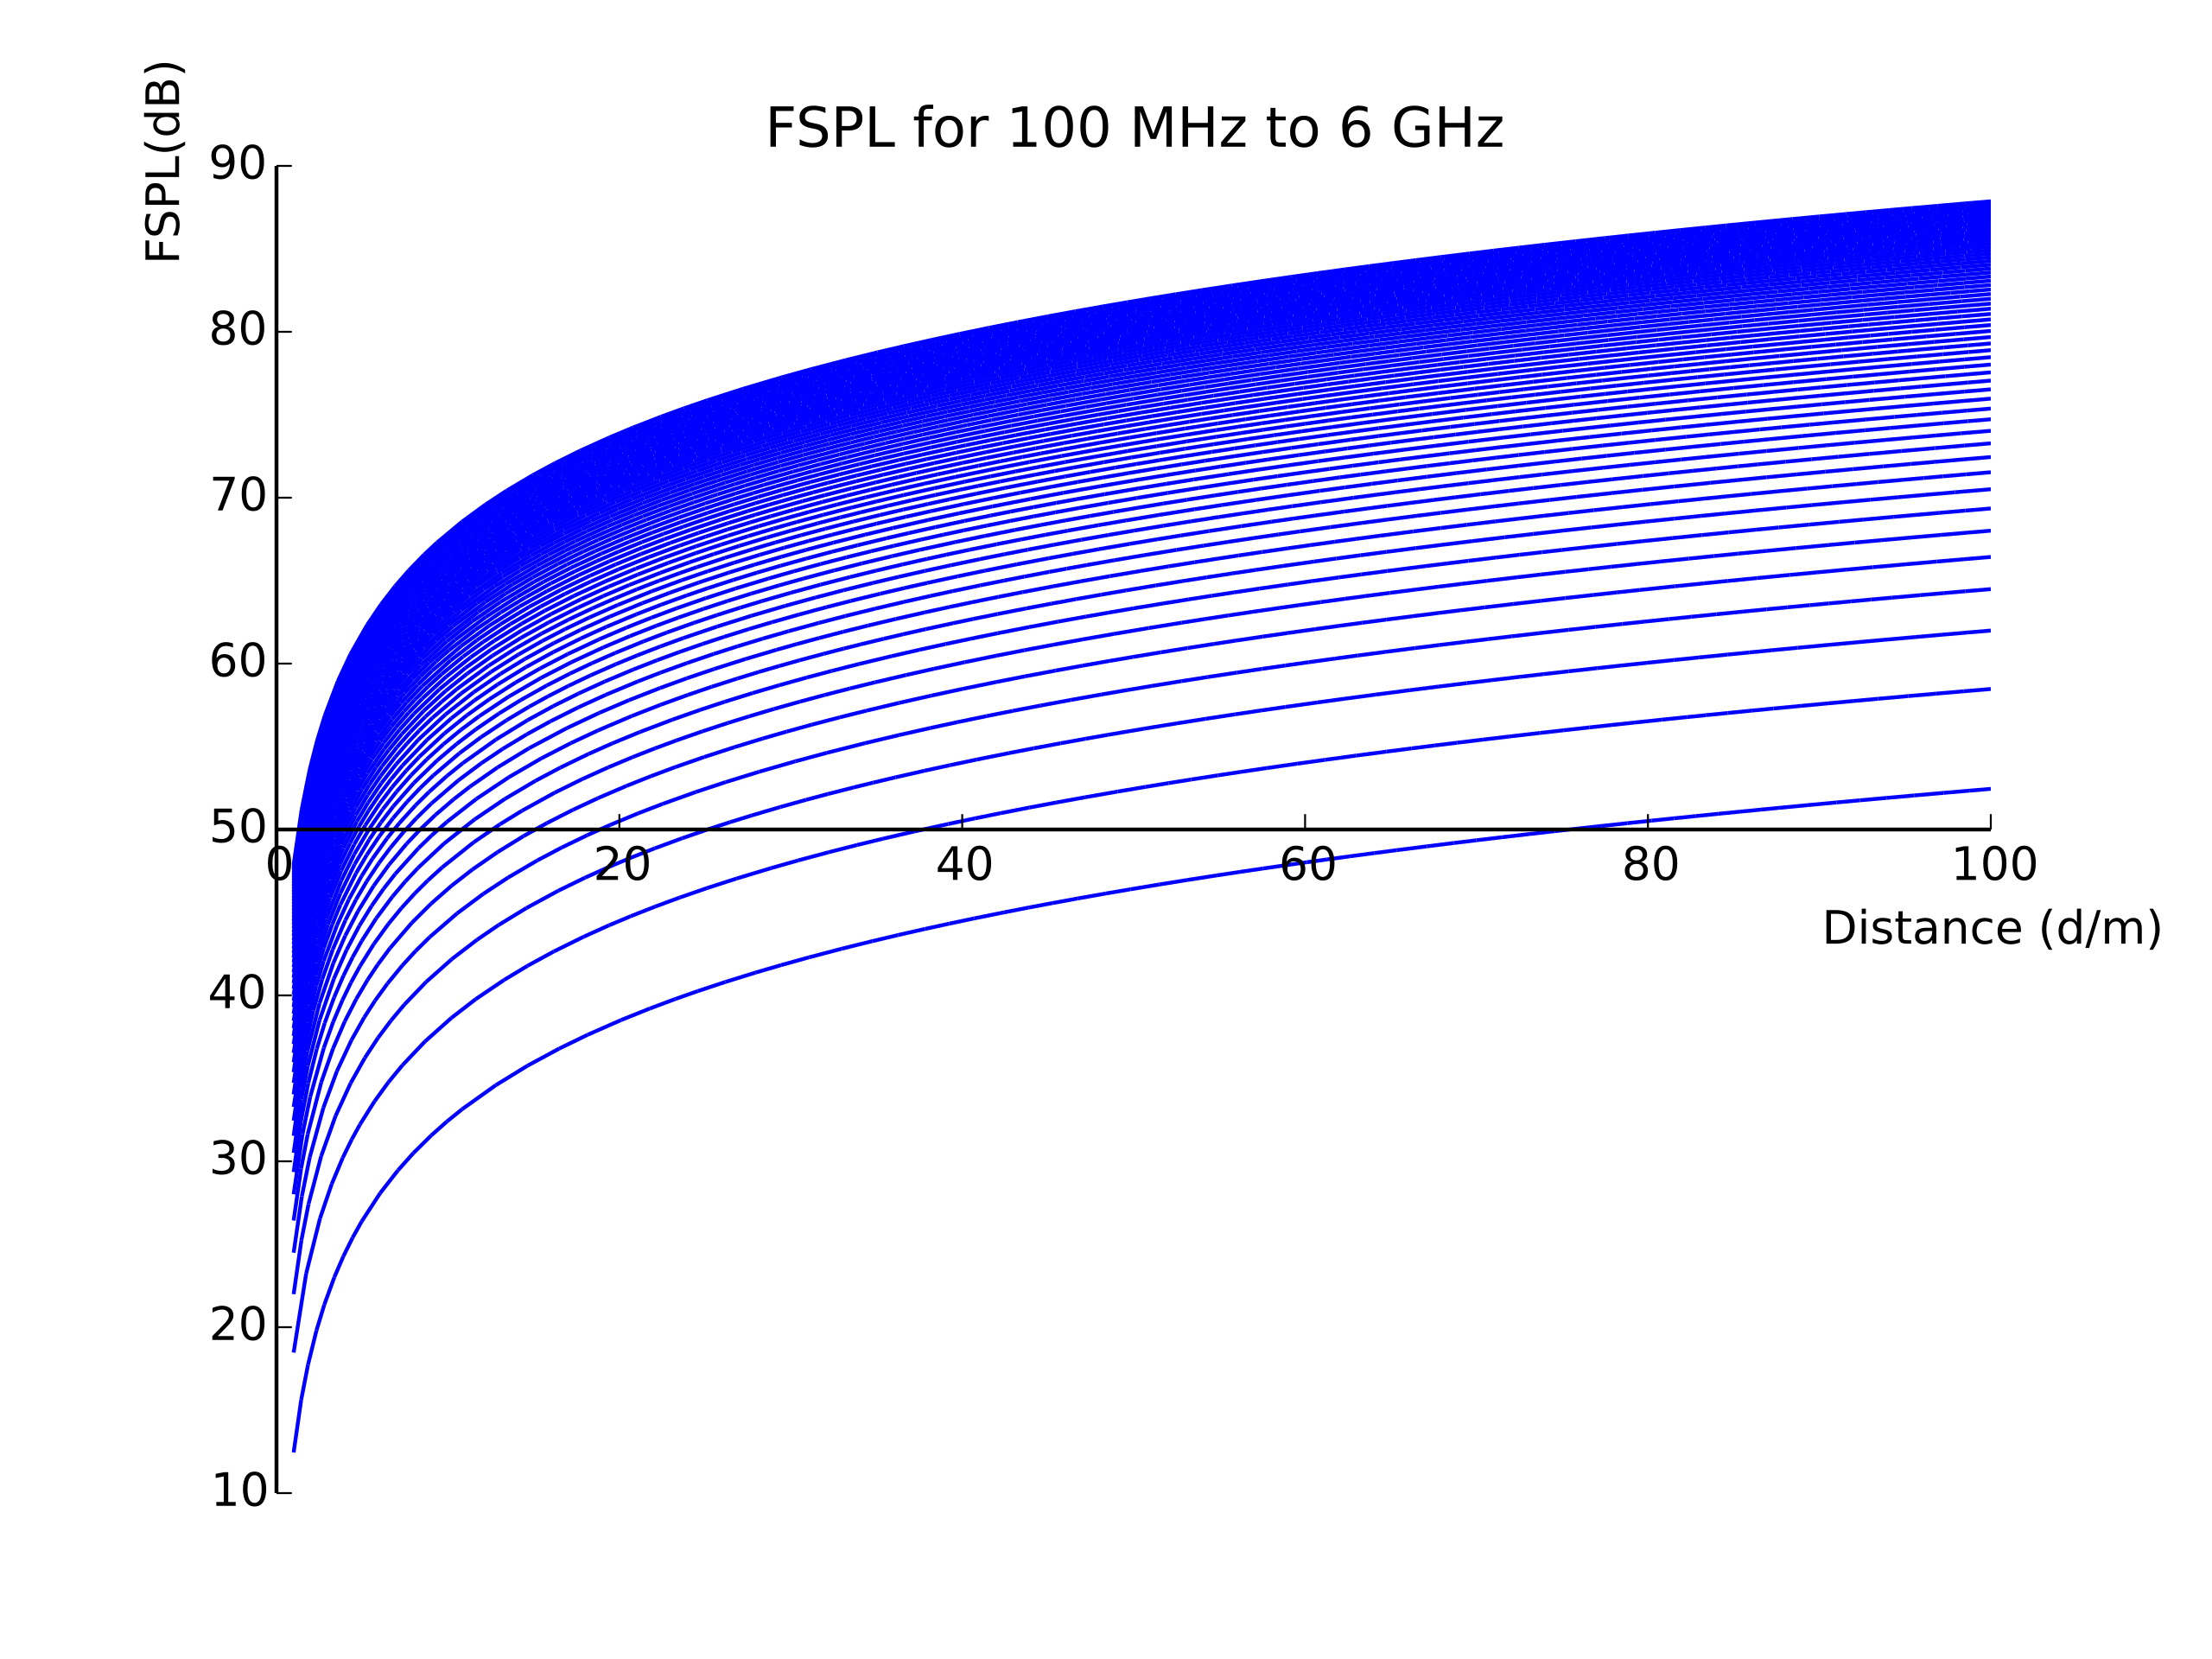
\includegraphics[width=0.9\textwidth]{./images/fspl_plot.png}

\section{Appendix A2: Streamlit App – Cell Coverage Planner}
\label{appendix:A2}
\textbf{URL:} \url{http://localhost:8501/CellCoverage} \\
\textbf{Features:} 
\begin{itemize}
    \item Adjust cell radius and visualize overlapping coverage.
    \item Frequency reuse simulation with color-coded hex cells.
    \item Path loss visualization with user-tunable exponent $n$.
\end{itemize}
